\documentclass[a4paper]{article}
\usepackage[english]{babel}
\usepackage[top=2cm,bottom=3cm,left=2.5cm,right=2.5cm]{geometry}
\usepackage[colorlinks=true, allcolors=black]{hyperref}
\usepackage{wrapfig} %문단 내 이미지 삽입
\usepackage[abs]{overpic} %이미지 위 텍스트 삽입
\usepackage{graphicx} %색상
\usepackage{mdframed} %글상자
\usepackage{titlesec} %섹션 이름 변경
\titlespacing*{\section}{0mm}{0mm}{0mm}
\titleformat{\section}{\bfseries\Large}{\Huge{\color{blue!60!green!80}\thesection}}{2ex}{}[]
\titlespacing*{\subsection}{0mm}{0mm}{0mm}
\titleformat{\subsection}{\bfseries}{\thesubsection\hspace{1ex}|}{1ex}{}[]
\usepackage[many]{tcolorbox}
\newcommand{\asw}[2]{
	\begin{flushright}
		{\color{blue!60!green}#1 \quad #2 \quad $\blacktriangleleft$}
	\end{flushright}
}
\newcommand{\pbox}[3]
{
	\begin{tcolorbox}[
		boxsep = 0mm,
		left = 3mm,
		right = 3mm,
		valign = center,
		colupper = black,
		colback = #1!70!black!15,
		colframe = #1!65!black,
		segmentation style = {
			double = #1!65!black,
			draw = #1!65!black,
			double distance=0.2mm,
			solid},
		after skip = 0mm
		]
		{\color{#1!65!black}#2}
		\ifx#3""\else\tcbline #3\fi
	\end{tcolorbox}
}
\newcommand{\cabox}[2]{\pbox{orange}{#1}{#2}}
\newcommand{\spbox}[2]{\pbox{green}{#1}{#2}}
\newcommand{\prbox}[2]{\pbox{blue!white!80}{#1}{#2}}
\newcommand{\lpbox}[2]{\pbox{magenta}{#1}{#2}}

\newcommand{\secbox}[1]{
	\begin{tcolorbox}[
		boxsep = 0mm,
		left = 4mm,
		right = 4mm,
		valign = center,
		colupper = blue!70!green!90,
		colback = blue!70!green!15,
		colframe = white,
		boxrule = 0mm
		]
		#1
	\end{tcolorbox}
}
\usepackage{amsmath, amsfonts, amssymb, bm} %수식
	\DeclareMathOperator{\arccsc}{arccsc}
	\DeclareMathOperator{\arcsec}{arcsec}
	\DeclareMathOperator{\arccot}{arccot}
	\DeclareMathOperator{\csch}{csch}
	\DeclareMathOperator{\sech}{sech}
	\DeclareMathOperator{\arcsinh}{arcsinh}
	\DeclareMathOperator{\arccosh}{arccosh}
	\DeclareMathOperator{\arctanh}{arctanh}
	\DeclareMathOperator{\arccsch}{arccsch}
	\DeclareMathOperator{\arcsech}{arcsech}
	\DeclareMathOperator{\arccoth}{arccoth}

	\DeclareMathOperator{\meter}{m}
	\DeclareMathOperator{\cm}{cm}
	\DeclareMathOperator{\mm}{mm}
	\DeclareMathOperator{\mum}{\mu m}
	\DeclareMathOperator{\newton}{N}
	\DeclareMathOperator{\kn}{kN}
	\DeclareMathOperator{\kgf}{kgf}
	\DeclareMathOperator{\pa}{Pa}
	\DeclareMathOperator{\kpa}{kPa}
	\DeclareMathOperator{\mpa}{MPa}
	\DeclareMathOperator{\gpa}{GPa}
	\DeclareMathOperator{\knpm}{kN/m}
	\DeclareMathOperator{\kph}{km/h}
	\DeclareMathOperator{\mps}{m/s}
	\DeclareMathOperator{\tkph}{kph}
	\DeclareMathOperator{\tmps}{mps}
	\DeclareMathOperator{\mpss}{m/s^2}
	\DeclareMathOperator{\dgr}{\!^\circ}
	\DeclareMathOperator{\cel}{\!^\circ C}
	\DeclareMathOperator{\kg}{kg}
	\DeclareMathOperator{\kgpcm}{kg/m^3}
	\DeclareMathOperator{\nm}{N\cdot m}
	\DeclareMathOperator{\kw}{kW}
	\DeclareMathOperator{\kwh}{kWh}
	\DeclareMathOperator{\mmhg}{mmHg}
	\DeclareMathOperator{\snd}{s}
\usepackage{polynom} %나눗셈 필산
\usepackage{cancel} %수식 약분선
\usepackage[normalem]{ulem}%취소선
\usepackage{array} %표
\usepackage{kotex} %한글

\title{
	\vspace{150pt}
	\textbf{\Huge Solutions}\\[10pt]
	of the Dynamics Midterm Exam 2023-1\\[20pt]
	\vspace{55pt}
	}
\author{E.Hong\vspace{90pt}}
\date{\today}

\begin{document}

\maketitle
\setlength{\parindent}{3mm}

\begin{center}
	\includegraphics[width=0.45\textwidth]{SSU symbol KR-EN.jpg}
\end{center}

\newpage

\spbox{\subsection*{Question 1}}
	{
	\begin{tabular}{m{50mm}m{95mm}}
	\includegraphics{img/001.png}
		& Knowing that the block $E$ is moving downward with a speed of $2\mps$, determine ($a$) the velocities of $C$ and $W$, ($b$) the relative velocity of $C$ with respect to $E$ and that of $W$ with respect to $E$.
	\end{tabular}
	}
	\vspace{\baselineskip}
	\begin{tabular}{m{70mm}m{75mm}}
		\includegraphics{img/002.png} &
		given :\quad$\mathbf{v}_{E} = 2\mps\downarrow$\newline\newline
		We can find some constraint equations.\newline\newline
		$d_C = 2d_E \quad\Rightarrow\quad v_C = 2v_E$\newline
		$d_W = d_E \quad\Rightarrow\quad v_W = v_E$\newline\newline
		$v_C = 2v_E = 4\mps$\newline
		$v_W = v_E = 2\mps$
	\end{tabular}
	\asw{($a$)}{$\mathbf{v}_C = 4.00\mps\uparrow\;;\;\mathbf{v}_W = 2.00\mps\uparrow$}
	\begin{align*}
		&v_{C/E} = v_C - v_E = 6\mps\\
		&v_{W/E} = v_W - v_E = 4\mps
	\end{align*}
	\asw{($b$)}{$\mathbf{v}_{C/E} = 6.00\mps\uparrow\;;\;\mathbf{v}_{W/E} = 4.00\mps\uparrow$}

\newpage

\spbox{\subsection*{Question 2}}
	{
	\begin{tabular}{m{49mm}m{96mm}}
		\includegraphics{img/003.png}
		& A 10-kg box $A$ and 20-kg box $B$ is sliding down the inclined conveyer belt in the position shown with speed $V_0$. Knowing that the coefficient of kinetic friction between $B$ and the belt is $0.3$, determine the minimum coefficient of static friction between $A$ and $B$ when $A$ does not slip on $B$.
	\end{tabular}
	}
		$$\text{given : \quad}\mu_k = 0.3,\quad m_A = 10\kg,\quad m_B = 20\kg$$
	In the system of $A$ and $B$, the FBD and KD is\\[5pt]
	\begin{tabular}{m{55mm}m{90mm}}
		\includegraphics{img/004.png}
		&
		$\displaystyle\sum F_y = 0$\newline\newline
		$N_{B/\text{belt}} - W_{AB}\cos20\dgr = 0$\newline
		$N_{B/\text{belt}} = (m_A+m_B)g\cos20\dgr$\newline
		$f_{B-\text{belt}} = \mu_kN_{B/\text{belt}} = \mu_k(m_A+m_B)g\cos20\dgr$\newline\newline
		$\displaystyle\sum F_x = ma$\newline\newline
		$W_{AB}\sin20\dgr - f_{B-\text{belt}} = (m_A+m_B)a$\newline
		$(m_A+m_B)g\sin20\dgr - \mu_k(m_A+m_B)g\cos20\dgr = (m_A+m_B)a$\newline
		$a = g(\sin20\dgr - \mu_k\cos20\dgr) = 0.589702\mpss$
	\end{tabular}\\[10pt]
	In the system of $A$, the FBD and KD is\\[10pt]
	\begin{tabular}{m{55mm}m{90mm}}
		\includegraphics{img/005.png}
		&
		$\displaystyle\sum F_y = 0$\newline\newline
		$N_{A/B} - W_A\cos20\dgr = 0$\newline
		$N_{A/B} = m_Ag\cos20\dgr$\newline\newline
		$\displaystyle\sum F_x = ma$\newline\newline
		$W_A\sin20\dgr - f_{A-B} = m_Aa$\newline
		$m_Ag\sin20\dgr - f_{A-B} = m_Ag(\sin20\dgr - \mu_k\cos20\dgr)$\newline
		$f_{A-B} = \mu_km_Ag\cos20\dgr$
	\end{tabular}
	\begin{align*}
		&f_{A-B}\leq \mu_sN_{A/B}\\
		&\mu_km_Ag\cos20\dgr\leq \mu_sm_Ag\cos20\dgr\\
		&\mu_k\leq \mu_s\\
		&\mu_{s,\text{min}} = \mu_k = 0.3
	\end{align*}
	\asw{}{$0.300$}

\newpage

\spbox{\subsection*{Question 3}}
	{
	\begin{tabular}{m{50mm}m{95mm}}
		\includegraphics{img/006.png}
		&
		A 40-Mg car $B$ is moving to the left in this picutre and combined with a 20-Mg car $A$ that is at rest. Knowing that the coefficient of friction between the wheels and ground is $0.3$ and the speed of $B$ just before combination is $4\mps$, determine ($a$) the velocity of $A$ and $B$ just after combining and ($b$) the time taken for them to stop.
	\end{tabular}
	}
	\begin{align*}
		\text{given :}\quad & v_B = 4\mps,\quad \mu_k = 0.3,\quad m_A = 20\times10^3\kg,\quad m_B = 40\times10^3\kg
	\end{align*}
	\begin{tabular}{m{85mm}m{65mm}}
		\includegraphics{img/007.png}
		&
		$p_0 = m_Bv_B = (m_A + m_B)v_{AB}$\newline\newline
		$\displaystyle v_{AB} = \frac{m_Bv_B}{m_A + m_B} = \frac{(40)(4)}{40+20}\mps $\newline\newline
		$\phantom{v_{AB}} = 2.67\mps$
	\end{tabular}
	\asw{($a$)}{$\mathbf{v}_{AB} = 2.67\mps\leftarrow$}
	\begin{align*}
		&F = \mu_kN = \mu_kg(m_A + m_B)\\
		&I = F\Delta t = \mu_kg(m_A + m_B)\Delta t\\
		&p_0 - I = 0\\
		&(m_A + m_B)v_{AB} - \mu_kg(m_A + m_B)\Delta t = 0\\
		&\Delta t = \frac{m_Bv_B}{\mu_kg(m_A + m_B)} = \frac{(40)(4)}{(0.3)(9.81)(40+20)}\snd = 0.906\snd
	\end{align*}
	\asw{($b$)}{$\Delta t = 0.906\snd$}

\newpage

\spbox{\subsection*{Question 4}}
	{
	\begin{tabular}{m{35mm}m{110mm}}
		\includegraphics{img/008.png}
		&
		A 1-kg block $B$ moving to the left with a speed $2\mps$ strikes a 0.5-kg ball $A$ that is hanging from a cord and is initially at rest. Knowing that the coefficient of kinetic friction between $B$ and the ground is $0.6$ and the coefficient of restitution between $A$ and $B$ is $0.8$, determine ($a$) the maximum $h$, ($b$) $x$ when $B$ stops.
	\end{tabular}
	}
	\vspace{\baselineskip}
	$v_A$, $v_B$, $v_A'$ and $v_B'$ are consumed as positive number when directions of velocities of them is left.
	\begin{align*}
		\text{given :}\quad & v_A = 0,\quad v_B = 2\mps,\quad m_A = 0.5\kg,\quad m_B = 1\kg,\quad \mu_k = 0.6,\quad e = 0.8\\
		&v_A' - v_B' = e(v_B - v_A)\\
		&v_A' - v_B' = ev_B\tag{1}\\
		&m_Av_A + m_Bv_B = m_Av_A' + m_Bv_B'\\
		&m_Bv_B = m_Av_A' + m_Bv_B'\tag{2}\\
		&\left\{\begin{array}{ll}
		v_A' - v_B' = ev_B & \qquad(1)\\
		m_Bv_B = m_Av_A' + m_Bv_B' & \qquad(2)
		\end{array}\right.\\
		&v_A' = \frac{m_B(e+1)}{m_A + m_B}v_B = \frac{(1)(0.8+1)}{0.5+1}(2\mps) = 2.4\mps\\
		&v_B' = v_A' - ev_B = (2.4\mps) - (0.8)(2\mps) = -0.8\mps
	\end{align*}\\[10pt]
	\includegraphics{img/009.png}
	\vspace{-32mm}\begin{align*}
		\text{we got :}\quad & v_A' = 2.4\mps,\quad v_B' = 0.8\mps\\
		&T_{A1} + V_{g,A1} = T_{A2} + V_{g,A2}\\
		&\frac{1}{2}m_A(v_A')^2 + 0  = 0 + m_Agh\\
		&h = \frac{(v_A')^2}{2g} = \frac{(2.4)^2}{2(9.81)}\meter = 0.294\meter
	\end{align*}
	\asw{($a$)}{$h = 0.294\meter$}
	\begin{align*}
		&T_{B1} + U_{B1\to B2} = T_{B2}\\
		&\frac{1}{2}m_B (v_B')^2 - \mu_km_Bgx = 0\\
		&x = \frac{(v_B')^2}{2\mu_k g} = \frac{(-0.8)^2}{2(0.6)(9.81)} = 0.0544\meter
	\end{align*}
	\asw{($b$)}{$x = 0.0544\meter$}




\end{document}